\documentclass[manuscript, letterpaper]{aastex6}

% to-do list
% ----------
% - check for TODO's and references to APW, HOGG, SMOH
% style notes
% -----------
% - This file generates by Makefile; don't be typing ``pdflatex'' or some bullshit.
% - Line break between sentences to make the git diffs readable.
% - Use \, as a multiply operator.
% - Reserve () for function arguments; use [] or {} for outer shit.
% - Use \sectionname not Section, \figname not Figure, \documentname not Article or Paper or paper.

\include{gitstuff}
% ----------------------------------- %
% start of AASTeX mods by DWH and DFM %
% ----------------------------------- %

\setlength{\voffset}{0in}
\setlength{\hoffset}{0in}
\setlength{\textwidth}{6in}
\setlength{\textheight}{9in}
\setlength{\headheight}{0ex}
\setlength{\headsep}{\baselinestretch\baselineskip} % this is 2 lines in ``manuscript''
\setlength{\footnotesep}{0in}
\setlength{\topmargin}{-\headsep}
\setlength{\oddsidemargin}{0.25in}
\setlength{\evensidemargin}{0.25in}

\linespread{0.54} % close to 10/13 spacing in ``manuscript''
\setlength{\parindent}{0.54\baselineskip}
\hypersetup{colorlinks = false}
\makeatletter % you know you are living your life wrong when you need to do this
\long\def\frontmatter@title@above{
\vspace*{-\headsep}\vspace*{\headheight}
\noindent\footnotesize
{\noindent\footnotesize\textsc{\@journalinfo}}\par
{\noindent\scriptsize Preprint typeset using \LaTeX\ style AASTeX6
with modifications by DWH and DFM.
}\par\vspace*{-\baselineskip}\vspace*{0.625in}
}%
\long\def\frontmatter@abstractheading{%
\makeaffils
  \vspace*{-\baselineskip}\vspace*{1.5pt}
  \vspace*{0.13189in}
 \begingroup
  \centering
  \abstractname
  \vskip 1mm
  \par
 \endgroup
 \everypar{\rightskip=0.0in\leftskip=\rightskip}\par
}%
\def\frontmatter@keys@format{\vspace*{0.5mm}%
  \settowidth{\keys@width}{\normalsize\@keys@name}%
  \rightskip=0.0in\leftskip=\rightskip\parindent=0pt%
    \hangindent=\keys@width\hangafter=1\normalsize\raggedright}%
\def\twodigits#1{\ifnum#1<10 0\fi\the#1}
\def\mydate{\leavevmode\hbox{\the\year-\twodigits\month-\twodigits\day}}
\makeatother
\renewcommand{\today}{\mydate}

% Section spacing:
\makeatletter
\let\origsection\section
\renewcommand\section{\@ifstar{\starsection}{\nostarsection}}
\newcommand\nostarsection[1]{\sectionprelude\origsection{#1}}
\newcommand\starsection[1]{\sectionprelude\origsection*{#1}}
\newcommand\sectionprelude{\vspace{1em}}
\let\origsubsection\subsection
\renewcommand\subsection{\@ifstar{\starsubsection}{\nostarsubsection}}
\newcommand\nostarsubsection[1]{\subsectionprelude\origsubsection{#1}}
\newcommand\starsubsection[1]{\subsectionprelude\origsubsection*{#1}}
\newcommand\subsectionprelude{\vspace{1em}}
\makeatother

\widowpenalty=10000
\clubpenalty=10000

\sloppy\sloppypar

% ------------------ %
% end of AASTeX mods %
% ------------------ %


% packages
\definecolor{cbblue}{HTML}{3182bd}
\usepackage{microtype}  % ALWAYS!
\usepackage{amsmath}
\hypersetup{backref,breaklinks,colorlinks,urlcolor=cbblue,linkcolor=cbblue,citecolor=black}

% define macros for text
\newcommand{\project}[1]{\textsl{#1}}
\newcommand{\acronym}[1]{{\small{#1}}}
\newcommand{\gaia}{\project{Gaia}}
\newcommand{\rave}{\project{\acronym{RAVE}}}
\newcommand{\apogee}{\project{\acronym{APOGEE}}}
\newcommand{\documentname}{\textsl{Article}}
\newcommand{\sectionname}{Section}
\newcommand{\figname}{Figure}
\newcommand{\eqname}{Equation}
\newcommand{\dr}{\acronym{DR1}}
\newcommand{\tgas}{\acronym{TGAS}}

% define macros for math
\newcommand{\given}{\,|\,}
\newcommand{\normal}{{\mathcal{N}}}
\newcommand{\dd}{\mathrm{d}}
\newcommand{\transp}[1]{{#1}^{\!\mathsf{T}}}
\newcommand{\inv}[1]{{#1}^{-1}}
\newcommand{\bs}[1]{\boldsymbol{#1}}
\newcommand{\vperp}{\bs{v}^\perp}
\newcommand{\propm}{\bs{\mu}}
\newcommand{\mat}[1]{\mathbf{#1}}
\renewcommand{\vec}[1]{\bs{#1}}
\newcommand{\kms}{\rm km~s^{-1}}
\newcommand{\msun}{{\rm M}_\odot}
\newcommand{\data}{\mathrm{data}}
\newcommand{\snr}{[S/N]_\varpi}
\newcommand{\eye}{\mathbb{I}}

% TODO
\newcommand{\todo}[1]{{\color{red}TODO: #1}}

\begin{document}\sloppy\sloppypar\raggedbottom\frenchspacing % trust me

\title{Co-moving stars in \textsl{Gaia DR1}}
\author{Semyeong Oh\altaffilmark{\pu,\lead},
        Adrian M. Price-Whelan\altaffilmark{\pu},
        David W. Hogg\altaffilmark{\ccpp,\mpia},
        Timothy D. Morton\altaffilmark{\pu},
        David N. Spergel\altaffilmark{\pu,\cca}
}

% Affiliations
\newcommand{\pu}{1}
\newcommand{\lead}{2}
\newcommand{\ccpp}{3}
\newcommand{\mpia}{4}
\newcommand{\cca}{5}

\altaffiltext{\pu}{Department of Astrophysical Sciences,
                   Princeton University, Princeton, NJ 08544, USA}
\altaffiltext{\lead}{To whom correspondence should be addressed:
                     \texttt{semyeong@astro.princeton.edu}}
\altaffiltext{\ccpp}{Center for Cosmology and Particle Physics,
                     Department of Physics,
                     New York University, 4 Washington Place,
                     New York, NY 10003, USA}
\altaffiltext{\mpia}{Max-Planck-Institut f\"ur Astronomie,
                     K\"onigstuhl 17, D-69117 Heidelberg, Germany}
\altaffiltext{\cca}{Simons Center for Computational Astrophysics, ...,
                    New York, NY XXXXX, USA}

\begin{abstract}
% Context
The primary sample of the \gaia\ \textsl{First Data Release} is the brand-new
\textsl{Tycho-Gaia Astrometric Solution}. The precision and size of this sample
creates an opportunity to find new binary stars and moving groups, especially
rare binaries or sparsely populated groups.
% Aims
Here we seize this opportunity.
% Methods
We use a justified marginalized likelihood ratio test to separate
pairs of stars with surprisingly similar three-space velocities from
those consistent with being drawn independently from the field
population.  Although we perform some visualizations using a
(bias-corrected) inverse parallax as a distance, the likelihood test
works in the observable space and uses the \gaia\ noise model
responsibly.
% Results
We find pairs of co-moving stars out to very wide
separations, including separations of a few parsecs! There does not
seem to be any tidal-disruption feature in the separation distribution
at sub-parsec scales. Pairs at separations beyond a
parsec---whether they are bound in a multiple system or drifting
apart---must be very short-lived. The photometric properties of the
members of these pairs are consistent with youth. The prospects for
testing stellar models and chemical abundance measurements are
superficially discussed.
\end{abstract}

\keywords{
  binaries: visual
  ---
  methods: statistical
  ---
  open clusters and associations: general
  ---
  parallaxes
  ---
  proper motions
  ---
  stars: formation
}

\section{Introduction} \label{sec:intro}

Two stars moving with similar full-space velocity vectors (``co-moving stars'')
are either members of a widely-separated stellar multiplet, or remnants of a
dispersing stellar system.

Widely-separated binary stars are weakly bound binary star systems with
semi-major axes larger than $a \gtrsim 10^{-3}~{\rm pc}$. It is generally
assumed that the stars in a wide binary form from gas with the same chemical
composition and are separated enough that there is no interaction or minimal
cross-pollution as the more massive star evolves (\citealt{todo}). Because the
binding energy of these systems is so low, if wide binary stars survive for many
Gigayears their existence alone places limits on the tidal field of the Galaxy
(\citealt{todo}) and the graininess of the gravitational field (\citealt{todo}).
In this picture, a remaining puzzle is how these systems survive the dense
stellar environments of the birth clusters in which they form. Wide binaries are
therefore important tools for studying small-scale star formation and the
large-scale Galactic mass distribution. These stars will appear to be co-moving
with velocity differences comparable to the binary orbital velocity at the
given separation.

At the largest separations, $a \gtrsim 1~{\rm pc}$, co-moving stars are likely
either remnants of disrupting stellar systems or young wide binary stars: at
these extreme separations, the Galactic tidal field would disrupt binary stars
within $t_{\rm disrupt} \lesssim XX~{\rm Gyr}$. Unbound open clusters with
velocity dispersions $\sigma_v \lesssim 1~\kms$ in the Galactic disk disrupt
quickly leaving small streams of stars with the same chemical abundances
(\citealt{chemicaltaggingstuff}). Disrupting or disrupted globular clusters and
dwarf galaxies also produce streams of stars with similar chemical properties
but with larger velocity differences (\citealt{streampeeps}). Stars from such
systems at similar orbital phases will appear to be co-moving with velocity
differences comparable to the internal velocity dispersions, $\sigma_v \approx
1$--$10~\kms$.

To date, thousands of candidate co-moving star pairs have been identified by
searching for stars with common proper motions (\citealt{Luyten:1979,
Poveda:1994, Allen:2000, Gould:2003, Chaname:2004, Lepine:2007,
Alonso-Floriano:2015}). \todo{how is our search different? (1) we have distance, (2) bigger volume than Hipparcos, (3) we use the data properly, (4) we don't cut on distance or on magnitude of proper motion -- we cut on parallax S/N}
% Cite:
% Tokovinin & Lepine 2012
% https://ui.adsabs.harvard.edu/#abs/2012ApJ...757..170A/abstract
% https://ui.adsabs.harvard.edu/#abs/2012AJ....144..102T/abstract
% https://ui.adsabs.harvard.edu/#abs/2014ApJ...790..158A/abstract

% Many searches find things close in angular separation, but need pms / distance

% Two stars moving with full-space velocity vector differences $\lesssim 1~\kms$
% with orbital semi-major axes $a \gtrsim 10^-3~{\rm pc}$.

Useful for:
- star cluster disruption and dispersal
- chemical abundance comparison (no interaction)
- dynamics

In either case, co-moving stars are of great interest
for studying the destruction of star clusters and dwarf galaxies, the tidal
field and small-scale properties of the mass distribution in the Milky Way, and
chemical uniformity and star formation processes.

\section{Data} \label{sec:data}

The primary data set used in this \documentname\ is the Tycho-Gaia Astrometric
Solution (\tgas), released as a part of Data Release 1 (\dr) of the Gaia mission
(\citealt{many}). \tgas\ contains astrometric measurements (sky position,
parallax, and proper motions) and associated covariance matrices for a large
fraction of the \project{Tycho-2} catalog (\citealt{tycho2}) with median
astrometric precision comparable to that of the \project{Hipparcos} catalog
($\approx 0.3~{\rm mas}$; \citealt{hipparcos}). In terms of parallax
signal-to-noise ($\snr = \varpi/\sigma_\varpi$), the \tgas\ catalog contains
42385 high-precision stars with $\snr > 32$: here we visualize quantities
computed from this high-precsision sample to emphasize the quality of the data.
In the sections that follow, we construct a statistical model that propagates
the non-trivial uncertainties in the data to our beliefs about the likelihood
that a given pair are co-moving.

For each star with $\snr > 32$, we use the reported parallax and parallax
error to compute a distance corrected for the Lutz-Kelker bias
(\citealt{lutzkelker}):
\begin{equation}
  d_{\rm LK} = 1000 \, \left[\frac{\varpi}{2} \,
    \left(1 + \sqrt{1 - \frac{16}{\snr^2}} \right) \right]^{-1} \, {\rm pc}
\end{equation}
We use this distance and the sky positions of each source to compute 3D
Cartesian positions, $\boldsymbol{x}$, for all stars and find the nearest
neighbor to each source in 3-space using the KDTree implementation in
\project{scikit-learn} (\citealt{scikit-learn}). We remove duplicates from
this sample and are left with 29870 pairs of stars. For all pairs, we then
compute the tangential velocity difference
\begin{equation}
  |\Delta \vec{v}_{\rm t}| = d_{\rm LK} \,
                            \sqrt{(\mu_{\alpha,1}-\mu_{\alpha,2})^2 +
                                  (\mu_{\delta,1}-\mu_{\delta,2})^2}
\end{equation}
\figname~\ref{fig:dv-sep} shows the tangential velocity difference against the
physical separation plotted for all pairs that pass the above signal-to-noise
cut. Pairs with small physical separation also tend to have small velocity
differences. Intriguingly, there appear to be an abundance of pairs with small
velocity separation at separations $|\delta\vec{x}| \gtrsim 1~{\rm pc}$. Of
course, this figure really only highlights close pairs with small angular
separations:
At large angular separations, the tangential velocity differences will be large
because of projection effects.
To select a more representative population of co-moving stars, we must instead
model the 3-space velocities of the stars given observations of just two
components.

\begin{figure*}[p]
\begin{center}
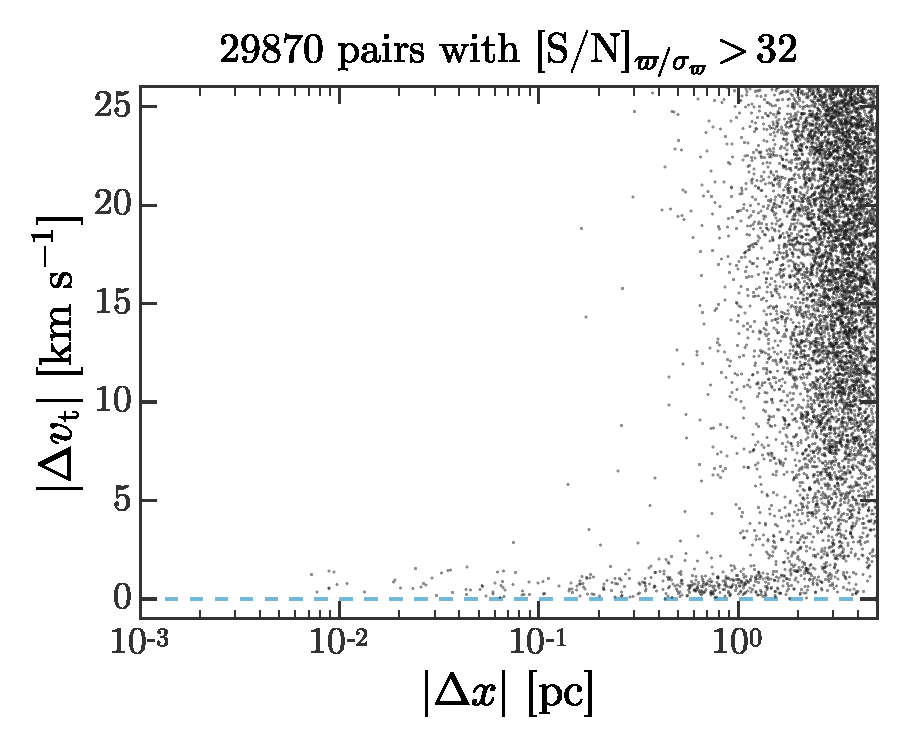
\includegraphics[width=\textwidth]{figures/dv-sep.pdf}
\end{center}
\caption{%
Difference in tangential velocity vs. physical separation for pairs of stars
selected to be nearest neighbors in separation. Dashed line shows zero velocity
difference. Note the points with small velocity difference: these are likely
widely-separated binary stars.
\label{fig:dv-sep}}
\end{figure*}

\section{Methods} \label{sec:methods}

The abundance of pairs of stars with small velocity difference in the
high-precision sample of \figname~\ref{fig:dv-sep} suggests that there are a
significant number of co-moving stars in the \tgas\ data at separations as large
as a few parsecs. Here we develop a method to select high-confidence co-moving
stars that properly incorporates the complex uncertainties associated with the
\gaia\ data. We make the following assumptions in order to construct a
statistical model (a likelihood function with explicit priors on our
parameters):
\begin{itemize}
  \item We assume that the uncertainties in the data---parallax, $\varpi$, and
    two proper motion components, $\propm = (\begin{array}[t]{c c} \mu_\alpha &
    \mu_\delta\end{array})^\mathsf{T}$---are Gaussian with known covariances
    $\mat{C}$.
    \todo{SMOH: mention GAIA paper that says Gaussian is good approximation?}
  \item We assume that the 3-space velocities of a given pair of stars
    $(\vec{v}_i, \vec{v}_j)$ in the \tgas\ sample (relative to the solar system
    barycenter) are either (1) co-moving with velocity drawn from a velocity
    prior $p(\vec{v})$ and  velocity difference drawn from a zero-mean Gaussian
    with velocity dispersion $s$, or (2) individually drawn from a velocity
    prior $p(\vec{v})$.
\end{itemize}

Under these assumptions, the likelihood of a proper motion measurement for a
star given true distance, $d$, and true tangential velocity, $\vec{v}^\perp =
(\begin{array}[t]{c c} v_\alpha & v_\delta\end{array})^\mathsf{T}$ is
\begin{align}
  L(\vec{v}, d, s^2) &=
    \left[\det\left(\frac{\tilde{\mat{C}}^{-1}}{2\pi}\right)\right]^{1/2} \,
    \exp \left[ -\frac{1}{2} \transp{\left(\vec{\mu} - \vec{x}_\theta \right)} \,
    \tilde{\mat{C}}^{-1} \,
    \left(\vec{\mu} - \vec{x}_\theta \right) \right] \label{eq:likefn} \\
  \vec{x}_\theta &= d^{-1} \, \vec{v}^\perp
\end{align}
where the tangential velocity $\vec{v}^\perp$ is related to the 3-space velocity
$\vec{v}$ through projection onto a tangent plane at a given star's sky position
$(\alpha, \delta)$
\begin{align}
  \vec{v}^\perp &= \mat{M}\,\vec{v} \\
  & = \left(
      \begin{array}{c c c}
        -\sin\alpha & \cos\alpha & 0 \\
        -\sin\delta \, \cos\alpha & -\sin\delta \, \sin\alpha & \cos\delta
      \end{array}
    \right) \,
    \left(\begin{array}{c} v_x \\ v_y \\ v_z \end{array}\right) \label{eq:transformation}
\end{align}
and the modified covariance matrix $\tilde{\mat{C}}$ is
\begin{equation}
  \tilde{\mat{C}} = \mat{C} + s^2 \, \eye
\end{equation}

We compute the fully marginalized likelihood (FML) that a given pair of stars
has the same 3-space velocity with a small velocity difference drawn from a
zero-mean Gaussian with variance $s^2$ (hypothesis 1, $\mathcal{L}_1$), and
the FML of the stars having different 3-space velocities (hypothesis 2,
$\mathcal{L}_2$).
We use the FML ratio $\mathcal{L}_1/\mathcal{L}_2$ as a scalar for selecting
candidate co-moving stars, as described below in more detail.
To compute these FMLs, the likelihood functions $L_i, L_j$ are marginalized
over true 3-space velocity and distance for each star in the pair $(i,j)$.
\begin{align}
  \mathcal{L}_1 &=
    \int \, \dd d_i \, \dd d_j \, \dd^3 \vec{v} \,
    L_i(\vec{v}, d_i, s^2) \,
    L_j(\vec{v}, d_j, s^2) \,
    p(\vec{v}) \, p(d_i \given \varpi_i) \, p(d_j \given \varpi_j) \\
  \mathcal{L}_2 &=
    \int \, \dd d_i \, \dd d_j \, \dd^3 \vec{v}_i \, \dd^3 \vec{v}_j \,
    L_i(\vec{v}_i, d_i, 0) \,
    L_j(\vec{v}_j, d_j, 0) \,
    p(\vec{v}_i) \, p(\vec{v}_j) \, p(d_i \given \varpi_i) \, p(d_j \given \varpi_j). \label{eq:hyp2}
\end{align}
The marginalization integral for hypothesis 2 can be split into the product of
two simpler integrals $\mathcal{L}_2 = Q_i \, Q_j$ where
\begin{equation}
  Q = \int \, \dd d \, \dd^3 \vec{v} \, L(\vec{v}, d, 0) \, p(\vec{v}) \, p(d\given\varpi)
\end{equation}
If the velocity prior $p(\vec{v})$ is also Gaussian, the integrals over velocity
in both cases can be performed analytically:
\todo{SMOH: is this what we do?}
We use an equal-weight mixture of three isotropic, zero-mean Gaussian
distributions
\begin{equation}
  p(\vec{v}) = \frac{1}{3} \, \sum_{m=1}^3 \, \mathcal{N}(0, \sigma_{v,m}^2)
\end{equation}
with velocity dispersions $(\sigma_{v,1}, \sigma_{v,2}, \sigma_{v,3}) = (8, 32,
128)~\kms$ meant to represent young disk stars, old disk stars, and halo stars.
We derive the relevant expressions in Appendix~\ref{sec:appendix}.
After marginalizing over velocity, the likelihood integrands only depend on
distance; we numerically compute the integrals over the true distances to each
star in a pair, $d_1,d_2$, using Monte Carlo integration with $K$ samples from
the distance posterior pdfs:
\begin{equation}
  \int \, \dd d \, \tilde{L}(d) \, p(d\given\varpi) \approx
    \frac{1}{K} \, \sum_k^K \, \tilde{L}(d_k)
\end{equation}
where $\tilde{L}(d)$ is the velocity-marginalized likelihood function.
Through experimentation, we have found that $K=128$ samples are sufficient for
estimating the above integrals for stars with a wide range in parallax
signal-to-noise.

\todo{APW/SMOH: in results, specify what we set $s^2$ to:}
To search for wide binaries, we set $s^2 = \frac{2 \, G \, \msun}{|\vec{x}_i-\vec{x}_j|}$.
To search for dissolving open clusters, we set $s^2 = 1~(\kms)^2$.

\section{Results 1: A catalog of candidate wide binaries}

\todo{Galactic context / orbits}

\section{Results 2: Star clusters and cluster remnants}

\section{Conclusions}

\acknowledgements

This research was partially supported by the \acronym{NSF} (grants
  \acronym{IIS-1124794}, \acronym{AST-1312863}, \acronym{AST-1517237}),
  \acronym{NASA} (grant \acronym{NNX12AI50G}),
  and the Moore-Sloan Data Science Environment at \acronym{NYU}. The data
analysis presented in this article was partially performed on computational
resources supported by the Princeton Institute for Computational Science and
Engineering (PICSciE) and the Office of Information Technology's High
Performance Computing Center and Visualization Laboratory at Princeton
University.

\software{The code used in this project is available from
\url{https://github.com/smoh/gaia-wide-binaries} under the MIT open-source
software license. This version was generated at git commit
\texttt{\githash\,(\gitdate)}.
This research additionally utilized:
    \texttt{Astropy} (\citealt{Astropy-Collaboration:2013}),
    %\texttt{emcee} (\citealt{Foreman-Mackey:2013}),
    \texttt{IPython} (\citealt{Perez:2007}),
    \texttt{matplotlib} (\citealt{Hunter:2007}),
    and \texttt{numpy} (\citealt{Van-der-Walt:2011}).}

% \facility{\sdssiii, \apogee}

\bibliographystyle{aasjournal}
\bibliography{refs}

\appendix

\section{Relevant properties of Gaussian integrals}
\label{sec:appendixA}

In what follows, all vectors are column vectors, unless we have transposed them.
A relevant exponential integral solution is
\begin{eqnarray}
  \ln\left[\int\exp(-\frac{1}{2}\,
    \transp{[\vec{x}-\vec{\nu}]} \,
    \inv{\mat{A}} \,
    [\vec{x}-\vec{\nu}] - \Delta) \, \dd \vec{x}\right]
  &=& +\frac{1}{2}\ln ||2\pi\,\mat{A}|| -\Delta
  \quad , \label{eq:gauss-int}
\end{eqnarray}
where $\vec{x}$ and $\vec{\nu}$ are $D$-dimensional vectors, $\mat{A}$ is a
positive definite matrix, $\Delta$ is a scalar, and the integral is over all of
$D$-dimensional $\vec{x}$-space.
To cast our problem in this form, we will need to complete the square of the
exponential argument.
If we equate
\begin{eqnarray}
  \frac{1}{2}\,\transp{[\vec{x}-\vec{\nu}]}\,\inv{\mat{A}}\,[\vec{x}-\vec{\nu}] + \Delta
  &=& \frac{1}{2}\,\transp{\vec{x}}\,\inv{\mat{A}}\,\vec{x} + \transp{\vec{x}}\,\mat{B}\,\vec{b} + C
  \quad ,
\end{eqnarray}
where $\mat{B}\,\vec{b}$ is an $D$-vector, and $C$ is a scalar, then we find
\begin{eqnarray}
  \vec{\nu} &=& -\mat{A}\,\mat{B}\,\vec{b}
  \\
  \Delta & = & C - \frac{1}{2}\,\transp{\vec{\nu}}\,\inv{\mat{A}}\,\vec{\nu}
  \quad .
\end{eqnarray}
We will identify terms in our likelihood functions with $\mat{A}$,
$\mat{B}\,\vec{b}$, and $C$, convert to $\vec{\nu}$ and $\Delta$ and compute
the marginalized likelihood using \eqname~\ref{eq:gauss-int}.

\section{Expressions for the marginalized likelihoods}\label{sec:appendix}

At given distance $d$, the velocity-marginalized likelihood can be computed
analytically using the expressions in Appendix~\ref{sec:appendixA}.
As described above, we use an isotropic, mixture-of-Gaussians prior on velocity
where the velocity dispersion of a given mixture component is $\sigma_{v,m}$ and
the 3-space variance tensor is $\mat{V}_m = \sigma_{v,m}^2 \, \eye$.
The likelihood for the data is also a Gaussian, as shown in
\eqname~\ref{eq:likefn}.
We will start by writing down expressions for the the likelihood multiplied by
the prior pdf for the velocities.
Here we slightly change the notation used in \sectionname~\ref{sec:methods} for
simplicity.

We construct a velocity-space data vector $y$ as follows:
\begin{equation}
  \vec{y} =
    \transp{\left(
      \begin{array}{c c c c}
        d_i\,\mu_{\alpha,i} &
        d_i\,\mu_{\delta,i} &
        d_j\,\mu_{\alpha,j} &
        d_j\,\mu_{\delta,j}
      \end{array}
    \right)}
\end{equation}
where again the subscripts $i,j$ refer to the indices of each star in the pair
and we have multiplied the observables (the proper motions) by the distances
$d_i, d_j$, which is permitted because we are conditioning on the distances.
Fundamentally, our hypothesis 1 model (the stars have the same velocity with a
small difference) is
\begin{equation}
  \vec{y} = \mat{M} \, \vec{v} + \mathrm{noise}
\end{equation}
where now the $4 \times 3$ transformation matrix $\mat{M}$ is a stack of the
transformation matrices for each star computed from the pair of sky positions
and using \eqname~\ref{eq:transformation}.
The noise (in the $y$ vector) is drawn from a $4 \times 4$ Gaussian with
block-diagonal covariance matrix, $\mat{\Sigma}$, constructed from the
covariance matrix of the observables, $\mat{C}_i, \mat{C}_j$, and the distances
$d_i, d_j$:
\begin{equation}
  \mat{\Sigma} = \left(
    \begin{array}{c c}
      d_i^2 \, \mat{C}_i & 0 \\
      0 & d_j^2 \, \mat{C}_j
    \end{array}
  \right)
\end{equation}

Given all these definitions, the likelihood function for hypothesis 1 is
\begin{eqnarray}
  p(\data \given \vec{v}, d_i, d_j) &=& d_i^2\,d_j^2\,
    \normal(\vec{y} \given \mat{M}\,\vec{v}, \mat{\Sigma}) \\
  \ln p(\data \given \vec{v}, d_i, d_j) &=& 2\,\ln d_i + 2\,\ln d_j
    -\frac{1}{2}\,\ln||2\pi\,\mat{\Sigma}|| \nonumber \\
    && \quad -\frac{1}{2}\,\transp{[\vec{y}-\mat{M}\,\vec{v}]}\,
      \inv{\mat{\Sigma}}\,
      [\vec{y}-\mat{M}\,\vec{v}]
  \quad ,
\end{eqnarray}
where the factor of $d_i^2\,d_j^2$ converts to units of one over \gaia\ data
from units of one over $y$, which includes the distances.

Now we multiply this likelihood with the velocity prior (here shown only for one
prior velocity mixture component) and complete the square.
In the original parameterization, we find:
\begin{eqnarray}
  \mat{A} &=& \inv{[\transp{\mat{M}}\,\inv{\mat{\Sigma}}\,\mat{M}+\inv{\mat{V}_m}]}
  \\
  \vec{\nu} &=& -\mat{A}\,\transp{\mat{M}}\,\inv{\mat{\Sigma}}\,\vec{y}
  \\
  \Delta &=& -2\,\ln d_i -2\,\ln d_j
    +\frac{1}{2}\,\ln||2\pi\,\mat{\Sigma}|| +\frac{1}{2}\,\ln||2\pi\,\mat{V}_m|| \nonumber \\
    && \quad +\frac{1}{2}\,\transp{\vec{y}}\,\inv{\mat{\Sigma}}\,\vec{y} -\frac{1}{2}\,\transp{\vec{\nu}}\,\inv{\mat{A}}\,\vec{\nu}
  \quad ,
\end{eqnarray}
which we plug in to \eqname~\ref{eq:gauss-int} to get the marginalized
likelihood conditioned on the two distances $d_i, d_j$.

The marginalized likelihood for the hypothesis 2 model (the stars have
independent velocities) is very similar.
In this case, the marginalized likelihood is a product of two independent
integrals $Q$, composed in the same way as the hypothesis 1 model but now for
each star individually, where
\begin{eqnarray}
  \vec{y} &=&
    \transp{\left(
      \begin{array}{c c}
        d\,\mu_{\alpha} &
        d\,\mu_{\delta}
      \end{array}
    \right)}
  \\
  \mat{\Sigma} &=& d^2 \, \mat{C}
  \\
\end{eqnarray}
and $\mat{M}$ is now the transformation matrix for one star. Then, again,
\begin{eqnarray}
  \mat{A} &=& \inv{[\transp{\mat{M}}\,\inv{\mat{\Sigma}}\,\mat{M}+\inv{\mat{V}_m}]}
  \\
  \vec{\nu} &=& -\mat{A}\,\transp{\mat{M}}\,\inv{\mat{\Sigma}}\,\vec{y}
  \\
  \Delta &=& -2\,\ln d_i -2\,\ln d_j
    +\frac{1}{2}\,\ln||2\pi\,\mat{\Sigma}|| +\frac{1}{2}\,\ln||2\pi\,\mat{V}_m|| \nonumber \\
    && \quad +\frac{1}{2}\,\transp{\vec{y}}\,\inv{\mat{\Sigma}}\,\vec{y} -\frac{1}{2}\,\transp{\vec{\nu}}\,\inv{\mat{A}}\,\vec{\nu}
  \quad ,
\end{eqnarray}
and
\begin{equation}
  Q = \frac{1}{2}\ln ||2\pi\,\mat{A}|| -\Delta \quad .
\end{equation}

\end{document}
